\section{Results and Discussion}
This section presents the strategies used to obtain high performing agent and the evaluation methodology applied to compare the Baseline controller, the proactive MLP architecture and the reactive 1DCNN approach.

\subsection{Training Convergence and Optimal Checkpoint Selection}

\begin{figure}[H]
    \centering
    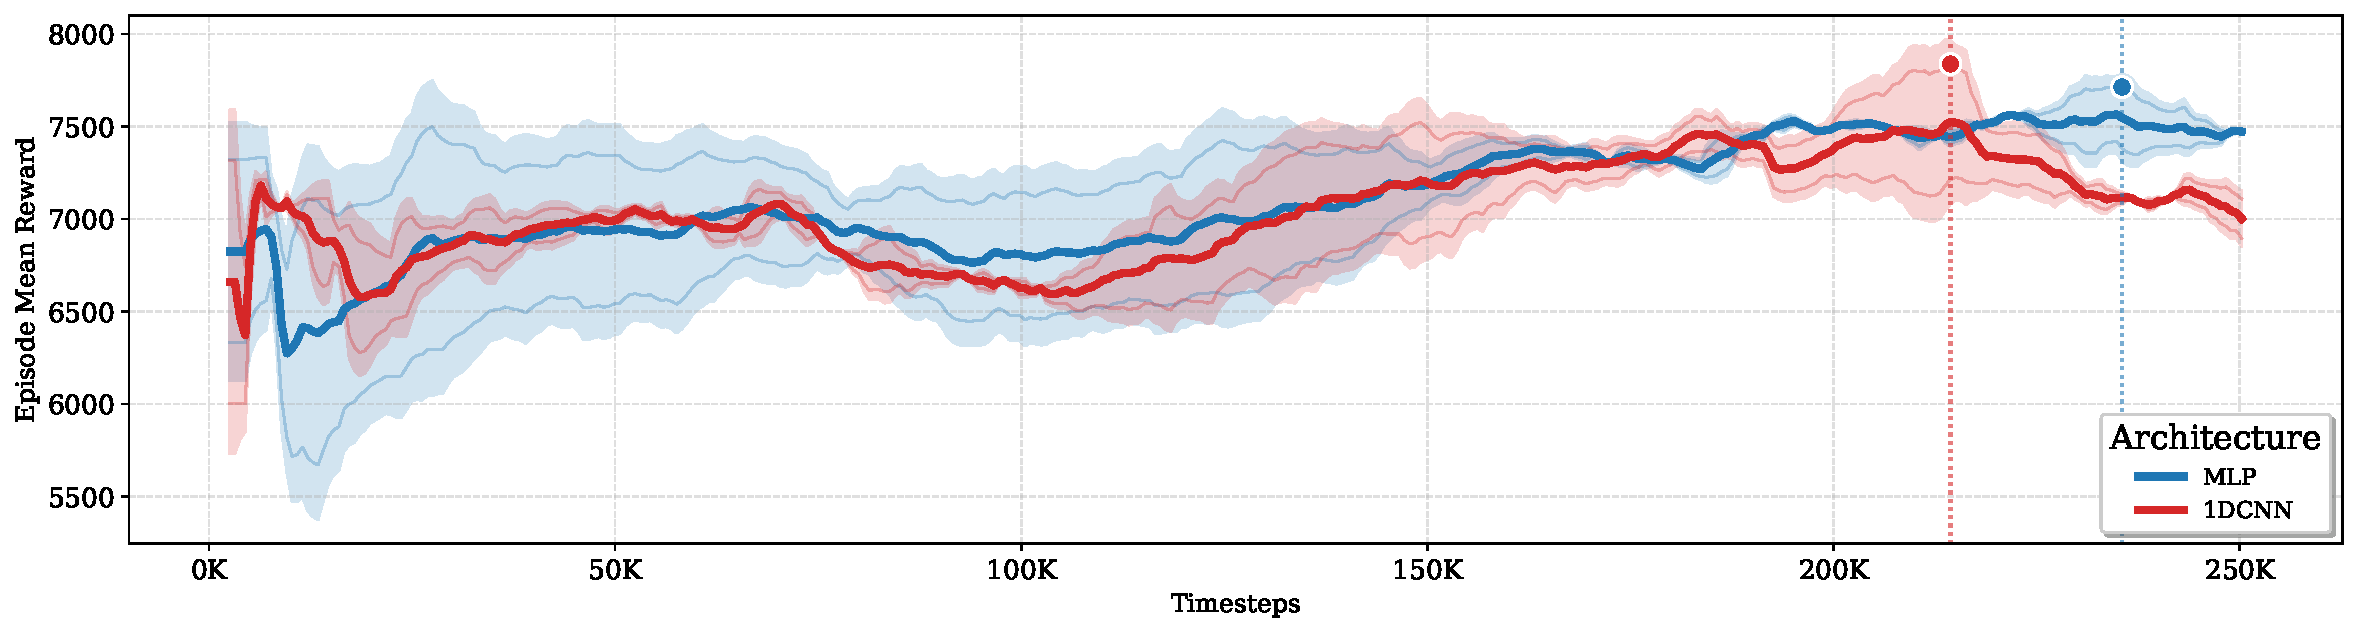
\includegraphics[width=1\linewidth]{resources/img/chapter4/ep_mean_reward.pdf}
    \caption{Training convergence and peak performance for MLP and 1DCNN architectures. Solid lines represent the exponential moving average (EMA, $\alpha=0.8$) of episode mean reward across all seeds. Shaded regions denote standard deviation ($\pm 1\sigma$), while faint trajectories correspond to individual runs. Vertical markers indicate peak performance checkpoints.}
    \label{fig:ep_mean}
\end{figure}

As illustrated in Figure~\ref{fig:ep_mean} both architectures shows a consistent upward trend in mean episodic reward, converging toward high performance plateaus exceeding $7{,}500$. The 1DCNN demonstrates improved early stage stability and reaches its peak reward faster (approximately $215$k timesteps) compared to the MLP baseline (approximately $235$k timesteps). To ensure reliable model selection two stage checkpoint selection procedure was applied: (i) identification of the maximum smoothed reward ($R_{\text{max}}$); (ii) temporal matching with the nearest saved checkpoint (stored at $5{,}000$-step intervals). The selected checkpoints were subsequently evaluated across diverse environmental conditions.

%; and (iii) downstream evaluation under standardized testing scenarios


\subsection{Evaluation Framework and Performance Metrics}
To evaluate generalization capabilities, both architectures were subjected to a deterministic evaluation suite across a combinatorial grid of 20 environmental configurations (Table \ref{tab:test_conditions}). These scenarios are categorized into three distinct regimes:

\begin{itemize}
    \item \textbf{Interpolation:} Headings of $95^{\circ}$, $115^{\circ}$, and $135^{\circ}$ assess stability within the primary training distribution.
    \item \textbf{Extrapolation:} Headings at $85^{\circ}$ and $145^{\circ}$ (positioned $5^{\circ}$ beyond the training boundaries) evaluate the graceful degradation of performance versus abrupt failure.
    \item \textbf{Stress Testing:} While wind speeds of 10, 14, and 18 knots represent trained conditions, the 20-knot scenario serves as a stress test to determine policy generalization under unobserved loads.
\end{itemize}

\begin{table}[htbp]
\centering
\caption{Evaluation Parameter Grid}
\label{tab:test_conditions}
\begin{tabular}{lc}
\hline
\textbf{Parameter} & \textbf{Testing Values} \\ \hline
Target Headings ($\theta_{target}$) & $85^{\circ}, 95^{\circ}, 115^{\circ}, 135^{\circ}, 145^{\circ}$ \\
Wind Speeds ($V_{wind}$) & $10, 14, 18, 20$ knots \\ \hline
\end{tabular}
\end{table}


\justify Feature normalization consistency was ensured by reloading the training-derived \texttt{VecNormalize} statistics. Performance was evaluated using multiple metrics: navigation precision (cross-track error and heading deviation), efficiency (CMG), and control stability (action slew rate). 

%This multidimensional evaluation framework enables detailed comparison of architectural resilience across varying environmental regimes.


\subsection{Steady-State Performance Comparison}
At the start of each navigation episode, the sailboat undergoes a transient phase before reaching stable dynamic behavior. To ensure a fair assessment of controller performance, these initial rising state were excluded from the analysis. Instead, steady state performance was evaluated using the tail segment of each episode where the control policy had converged to stable behavior. The steady state CMG was computed as

\begin{equation}
\mathrm{CMG}_{\text{steady}} = \frac{1}{T} \sum_{i = 201}^{512} \mathrm{CMG}_i,
\end{equation}

\justify where the first 200 timesteps were discarded to remove transient effects and $T = N - 200$ denotes the number of samples used for steady state averaging. Figure\ref{fig:cmg_bars} shows the $\mathrm{CMG}_{\text{steady}}$ comparison across test cases in Table \ref{tab:test_conditions}.

\begin{figure}[H]
    \centering
    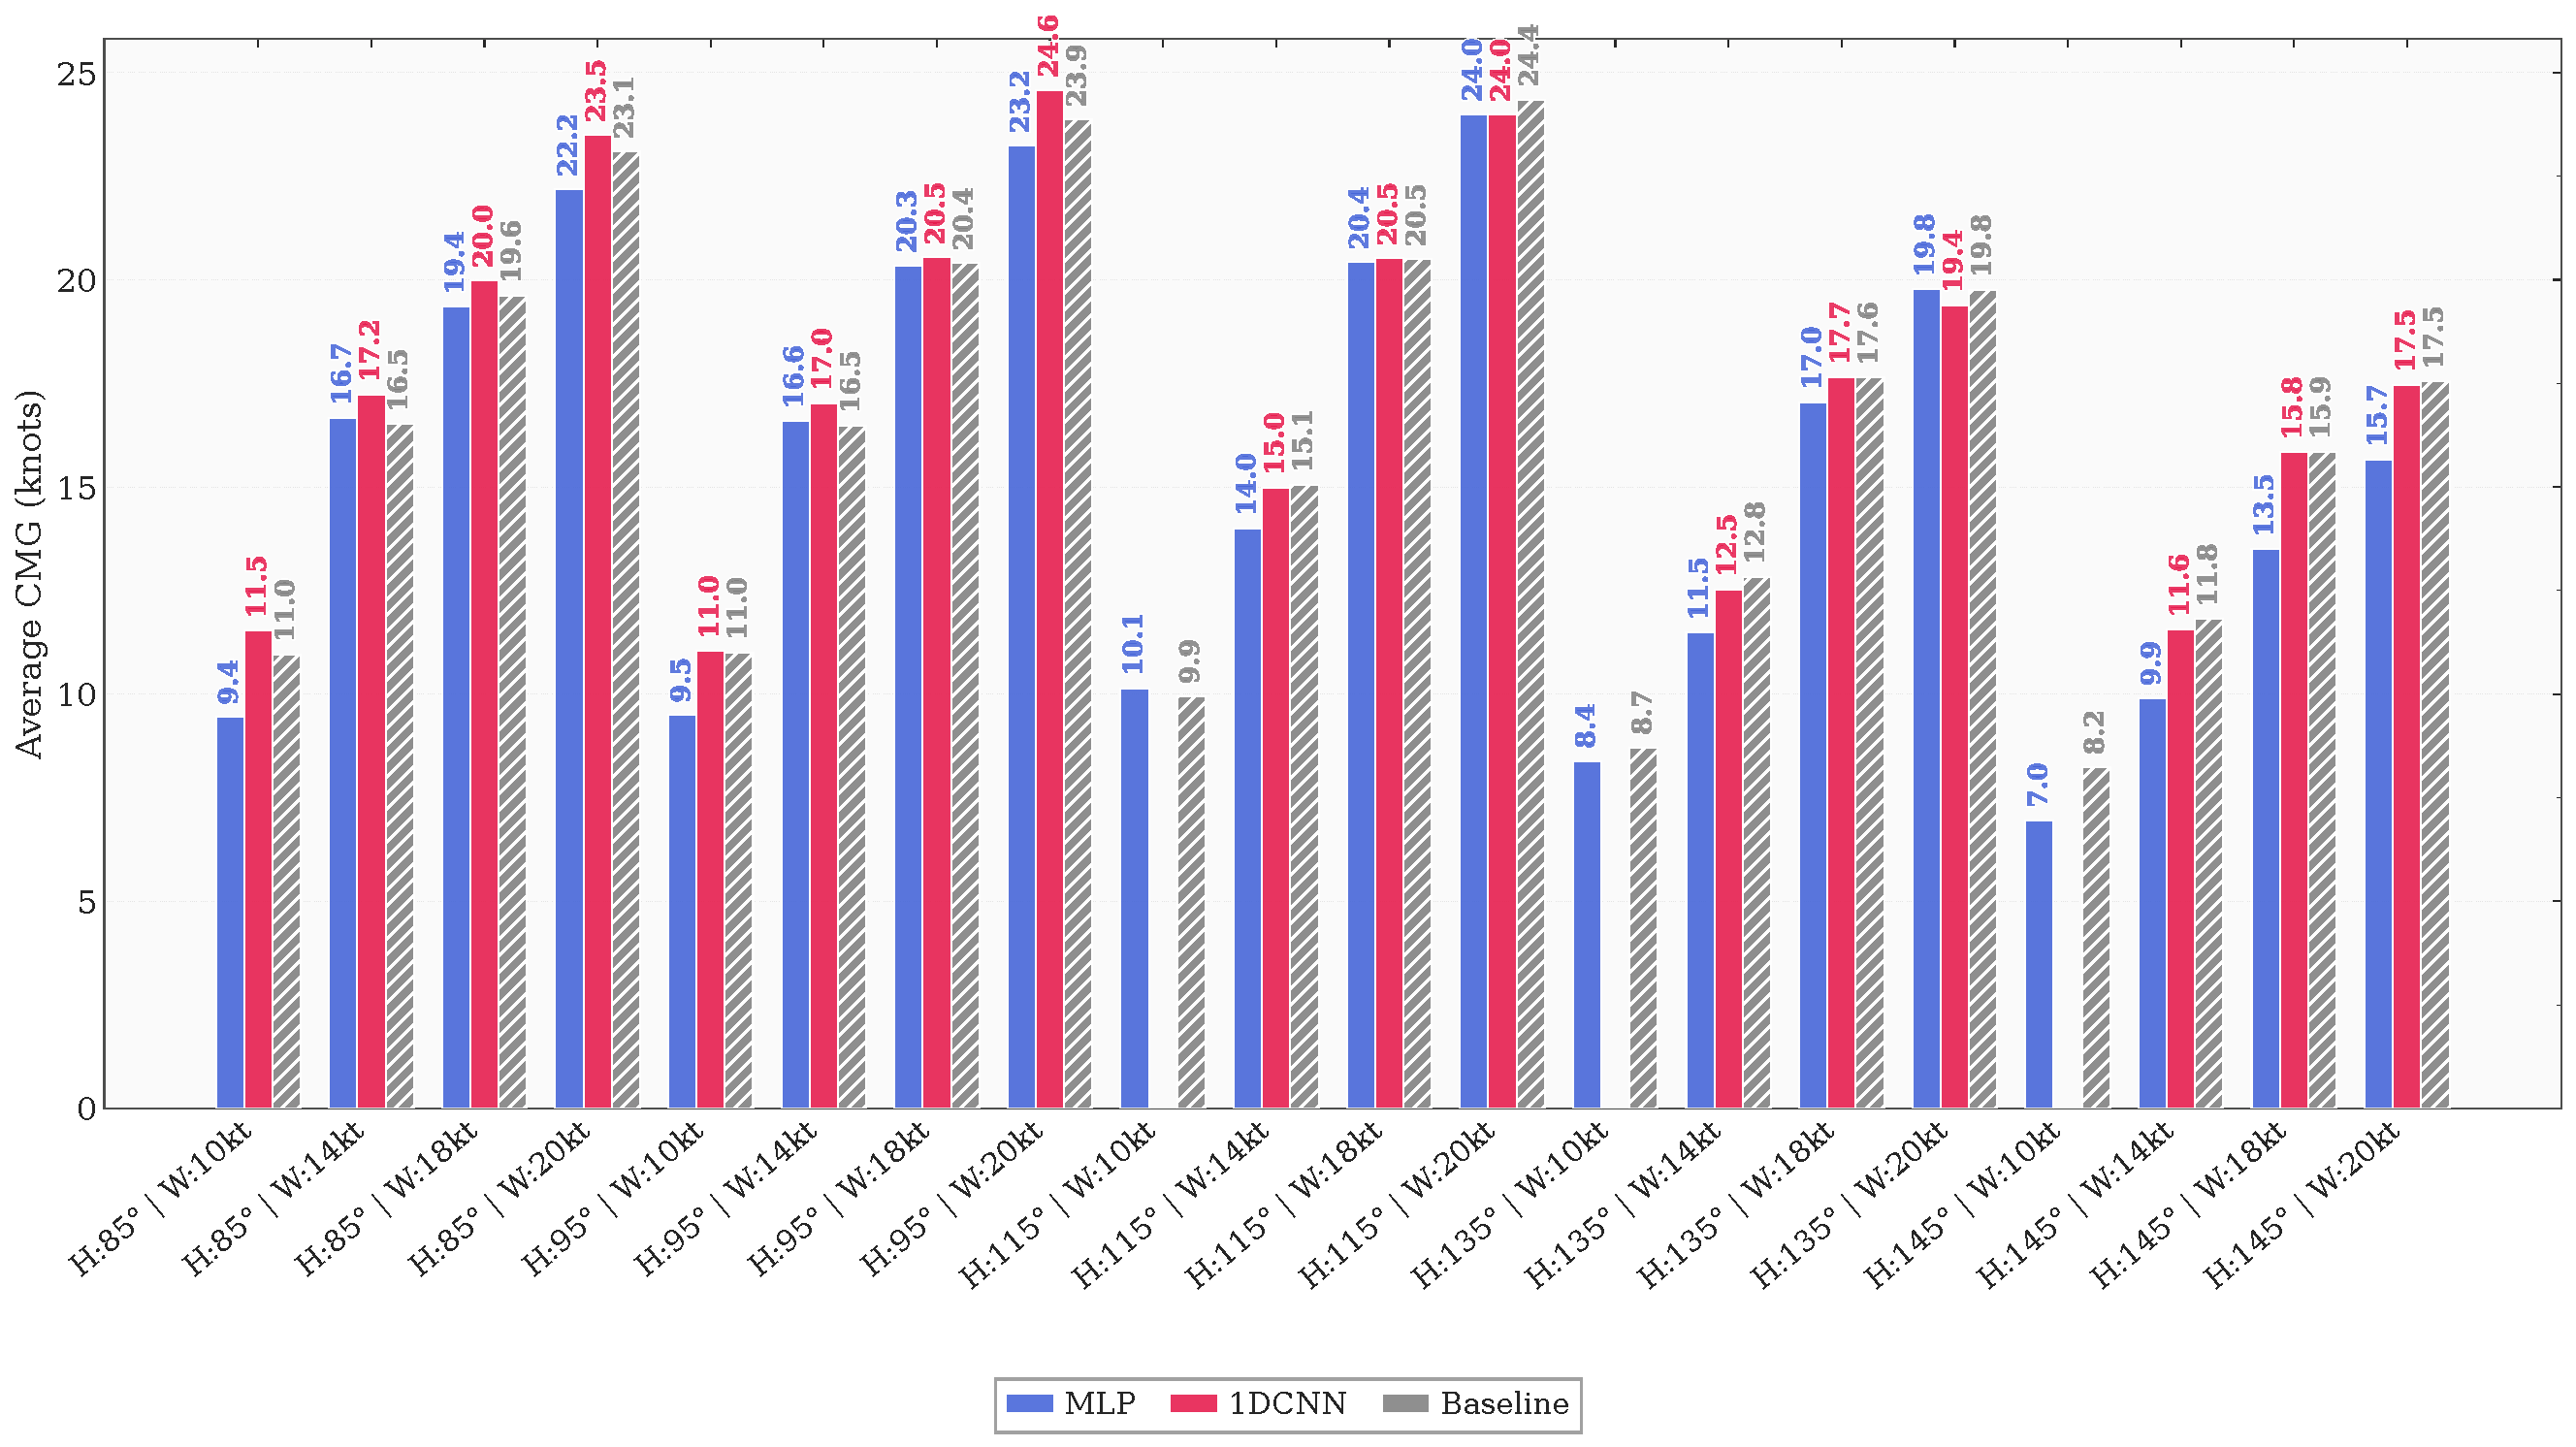
\includegraphics[width=1\linewidth]{resources/img/chapter4/per_case_cmg_comparison_pub.pdf}
    \caption{Steady-state CMG comparison across test cases. Performance differences are highlighted for out-of-distribution wind speeds ($20\,\text{kts}$) and boundary headings ($85^\circ$, $145^\circ$).}
    \label{fig:cmg_bars}
\end{figure}

 
\justify As shown in Figure~\ref{fig:cmg_bars}, both RL architectures generally outperform the baseline PID controller, which consistently achieves the lower bounds of CMG across the majority of test cases (e.g., 11.0\,kts at $H\!:\!85^\circ \mid W\!:\!14\,\text{kt}$ compared to 17.2\,kts for the 1DCNN and 16.7\,kts for the MLP). Both RL agents demonstrate strong performance and clear generalization beyond the training envelope ($H \in [90^\circ,140^\circ]$, $W \in [10,18]\,\text{kts}$). The 1DCNN emerges as the superior architecture for high-performance regimes, achieving the peak observed CMG of 24.6\,kts at $H\!:\!95^\circ \mid W\!:\!20\,\text{kt}$. Notably, the MLP exhibits significant performance degradation and policy instability under higher wind loads (18--20\,kts), whereas the 1DCNN maintains stable operation at these higher limits.
\justify However, a critical edge-case failure was identified for the 1DCNN in light-wind conditions (10\,kts) at headings $H\!:\!115^\circ$, $H\!:\!135^\circ$, and $H\!:\!145^\circ$. In these scenarios, the 1DCNN policy frequently leads to ``Out-of-Bounds'' (OOB) conditions, resulting in prematurely terminated episodes and lower average CMG values (e.g., 7.7\,kts at $H\!:\!135^\circ \mid W\!:\!10\,\text{kt}$) compared to the MLP (8.4\,kts) and baseline controller (8.7\,kts). This suggests that while the 1DCNN's temporal feature extraction excels at maximizing velocity under high loads, it may over-correct in low-energy states where the physical limits of the foils provide less damping. The polar distribution in Figure~\ref{fig:polar_plots} confirms that while the 1DCNN extends the performance frontier in the $120^\circ$ to $150^\circ$ heading range at high speeds, the MLP remains a more resilient, albeit less efficient, ``fail-safe'' option in marginal conditions.


\begin{figure}[h]
    \vspace{-3pt}
    \centering
    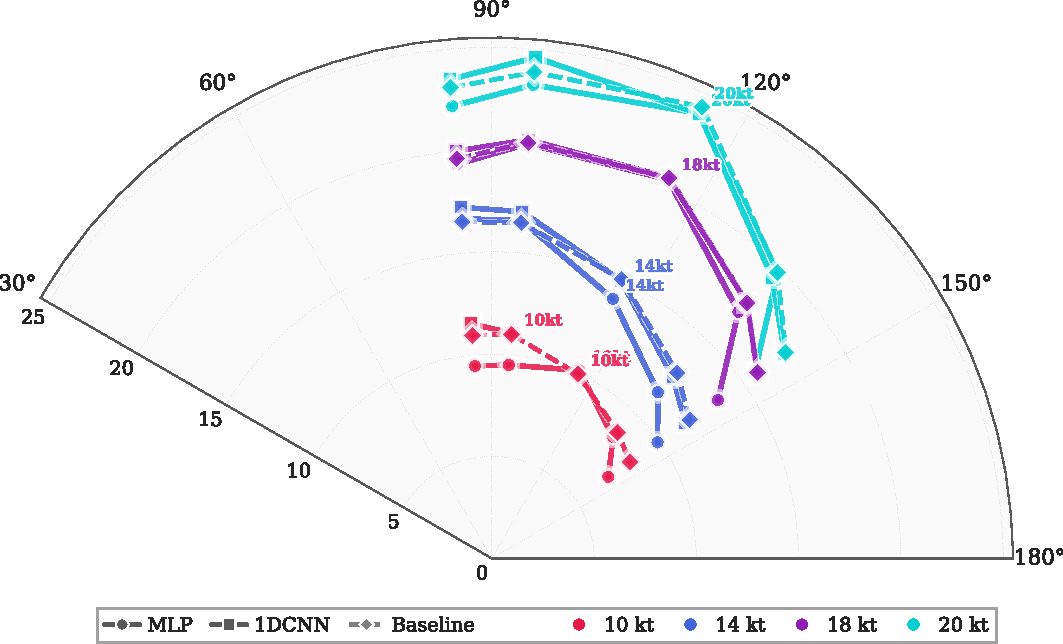
\includegraphics[width=1\linewidth]{resources/img/chapter4/polar_performance_pub.pdf}
    \caption{Polar performance distribution illustrating operational efficiency across headings. The 1DCNN maintains a broader and more consistent operational envelope.}
    \label{fig:polar_plots}
\end{figure}


\subsection{Control Dynamics and Temporal Stability}
\begin{figure}[h]
    \centering
    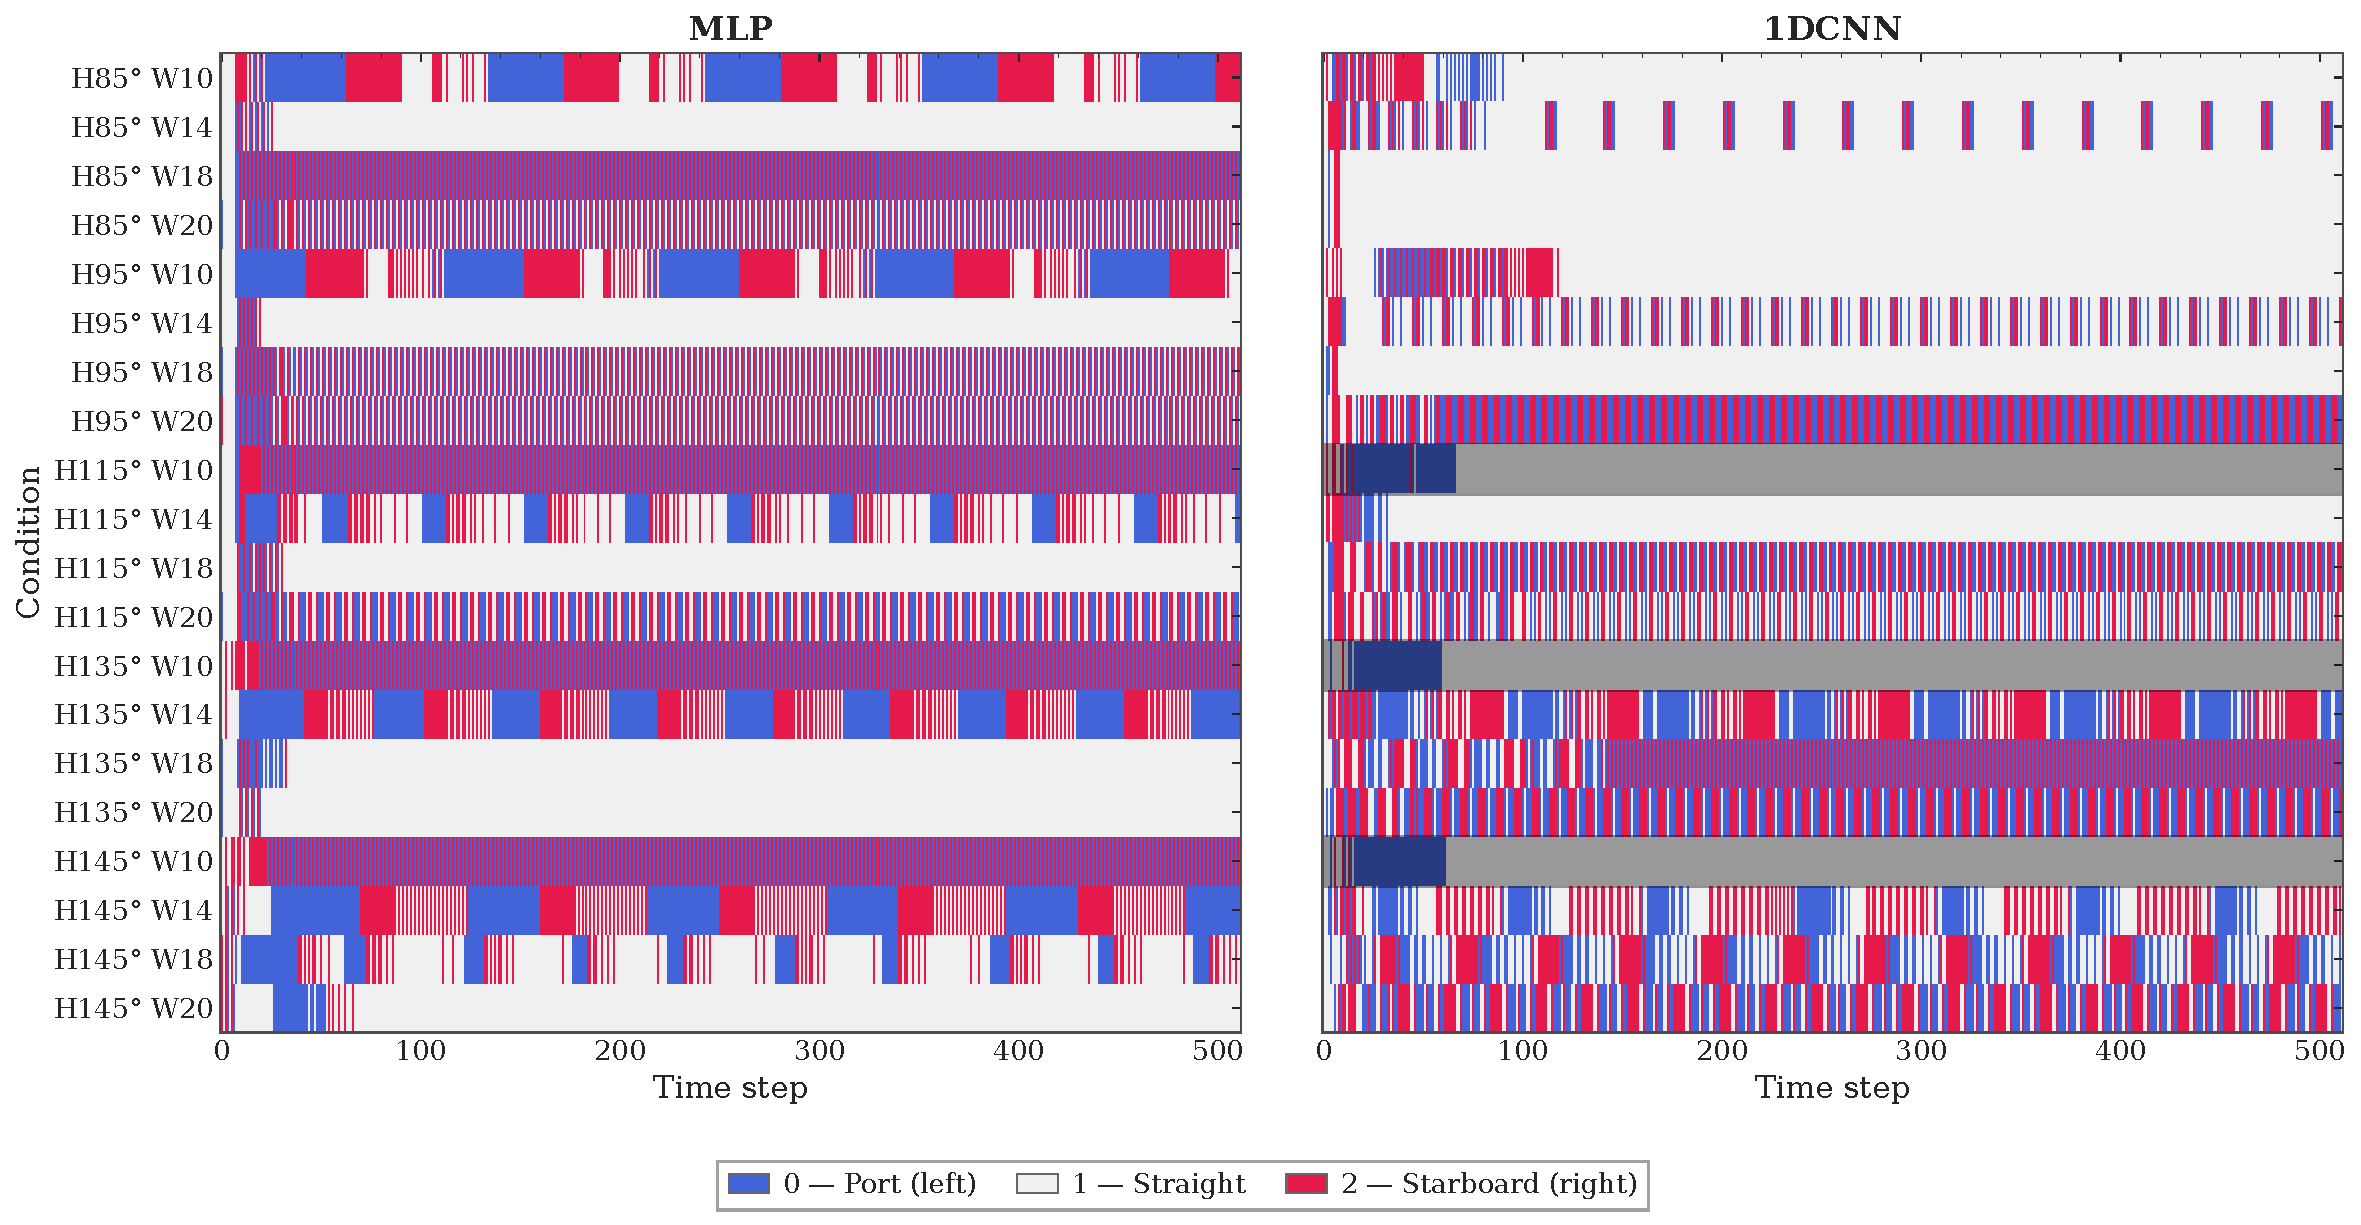
\includegraphics[width=1\linewidth]{resources/img/chapter4/action_heatmap_pub.pdf}
    \caption{Spatiotemporal heatmap of steering action offsets for MLP (left) and 1DCNN (right) across varying heading (H) and wind (W) conditions. The color gradient represents the difference between consecutive actions ($\Delta a_t = a_t - a_{t-1}$), where 0 (white) indicates a maintained course and 2 (dark red/blue) indicates maximum rudder deflection.}
    \label{fig:offsetmap}
\end{figure}

\justify To analyze the behavioral characteristics of the learned policies, we examine the action offset, defined as the numerical difference between the agent's current action and its previous action ($\Delta a_t = a_t - a_{t-1}$). This metric serves as a proxy for control \emph{jitter}: a high frequency of large offsets indicates aggressive or unstable steering behavior, whereas a concentration of small or zero offsets suggests smoother, more damped control resembling traditional PID-based steering. The command heatmaps in Figure~\ref{fig:offsetmap} reveal distinct operational signatures between the architectures across the 512-step evaluation episodes. The Multi-Layer Perceptron (MLP) exhibits pronounced policy instability, characterized by frequent high-magnitude offsets oscillating between port and starboard extremes. This ``chatter'' suggests that the MLP responds primarily to instantaneous environmental fluctuations without effectively leveraging temporal context, particularly near operational boundaries where maintaining stability becomes challenging.
\justify In contrast, the 1DCNN demonstrates a structured form of \emph{adaptive jitter}. Under high-wind conditions (14--20\,kts), steering corrections are concentrated around small-magnitude offsets, enabling the agent to maintain optimal foil lift and aerodynamic alignment while avoiding the large, energy-dissipating rudder oscillations observed in the MLP. However, this proactive control strategy introduces a trade-off in light-wind regimes (10\,kts). At headings H:115$^\circ$, H:135$^\circ$, and H:145$^\circ$, the 1DCNN's micro-correction behavior can lead to ``Out-of-Bounds'' (OOB) failures, as insufficient wind pressure limits the physical damping of steering inputs. These results indicate that while temporal feature extraction in the 1DCNN significantly enhances robustness and performance under high-load conditions, its aggressive optimization may reduce stability in marginal environments where the vessel operates near physical limits. This highlights a key design consideration for autonomous foiling controllers: balancing proactive performance optimization with fail-safe reactive mechanisms during low-energy operating states.


\subsection{Trajectory Analysis}
\begin{figure}[h]
    \centering
    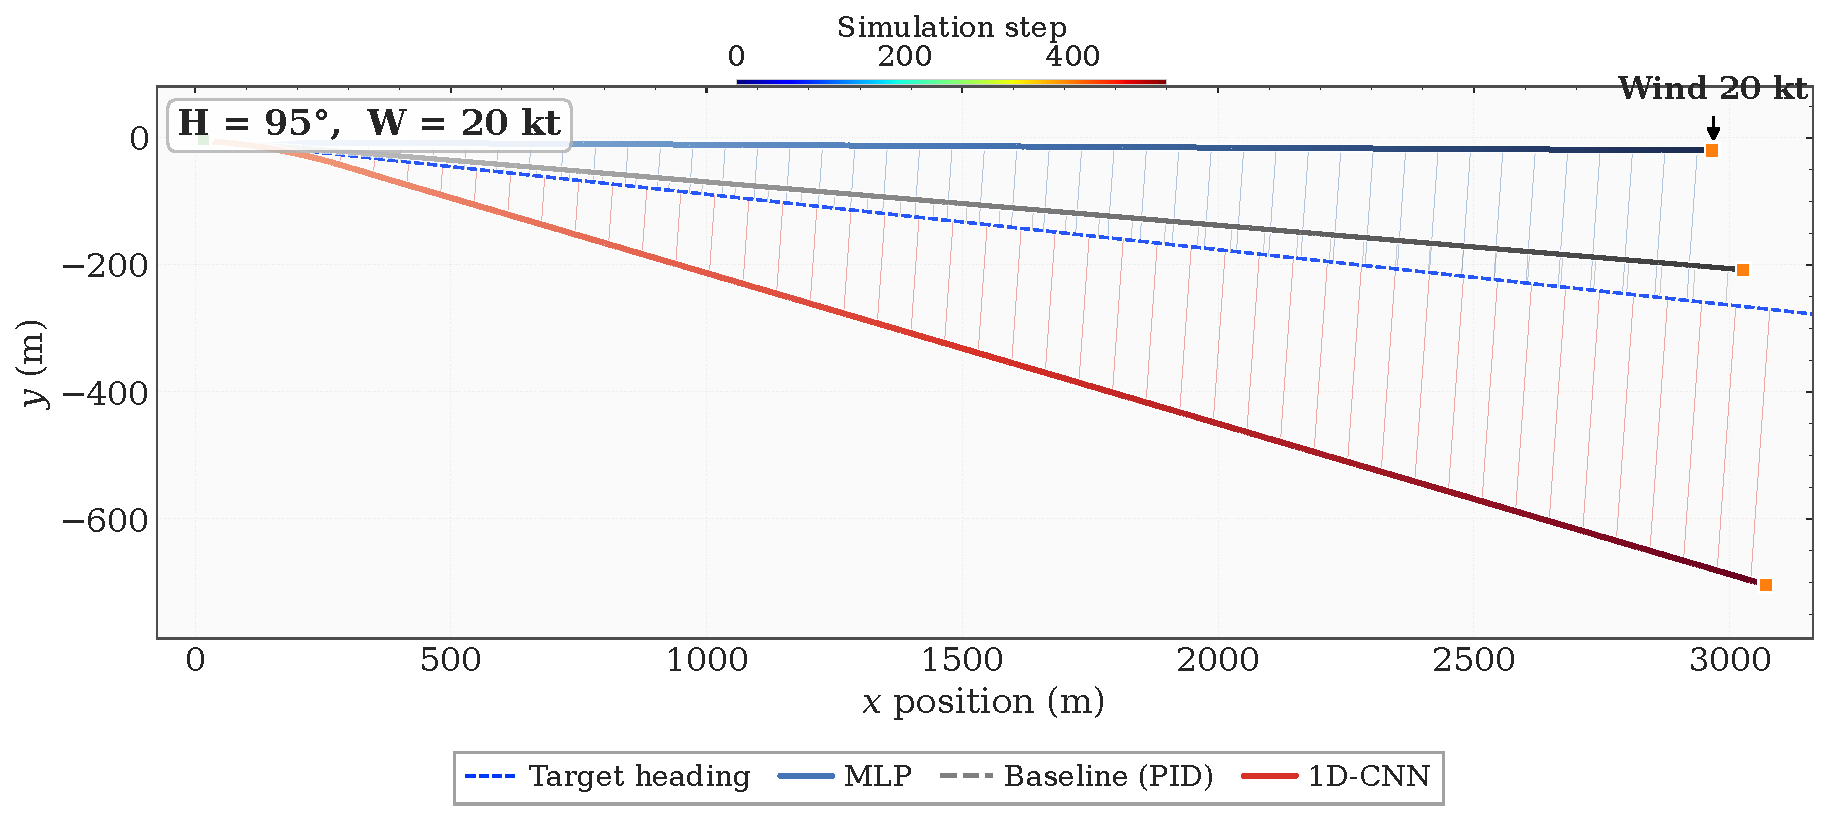
\includegraphics[width=0.9\linewidth]{resources/img/appendix/trajectory_samp.pdf}
    \caption{Distribution of action offsets ($\Delta a_t$) for MLP and 1DCNN across all test cases. The 1DCNN's distribution is more concentrated around zero, indicating smoother control, while the MLP exhibits a wider spread, reflecting higher jitter.}
    \label{fig:2dtrajectory}
\end{figure}

\justify The 2D trajectory plots (Figure~\ref{fig:2dtrajectory}) illustrate the spatial manifestations of the control policies discussed in the preceding sections. Under the boundary heading condition (H:85$^\circ$), the Baseline PID controller maintains a highly linear path but lacks proactive lift management, resulting in lower velocity and sub-optimal drift with the longest time-to-target. The MLP exhibits low-frequency oscillations in light-wind scenarios (W:10\,kt), producing a ``wavy'' trajectory that reflects the instability observed in the action-offset heatmaps, leading to increased drag and inefficient distance covered. In contrast, the 1DCNN demonstrates superior trajectory discipline, particularly under high-wind stress tests ($W{:}20\,\text{kt}$), maintaining the most direct and stable line toward the target by using ``adaptive jitter'' to make micro-adjustments and prevent the large-scale deviations seen in the MLP. While the 1DCNN can experience abrupt termination in low-wind edge cases due to OOB failures, its performance under viable foiling conditions remains the most robust and energy-efficient among the controllers.
